\section{Spark::Sp\-Matrix4$<$ Real $>$ Class Template Reference}
\label{classSpark_1_1SpMatrix4}\index{Spark::SpMatrix4@{Spark::SpMatrix4}}
{\tt \#include $<$Sp\-Matrix.h$>$}

Inheritance diagram for Spark::Sp\-Matrix4$<$ Real $>$:\begin{figure}[H]
\begin{center}
\leavevmode
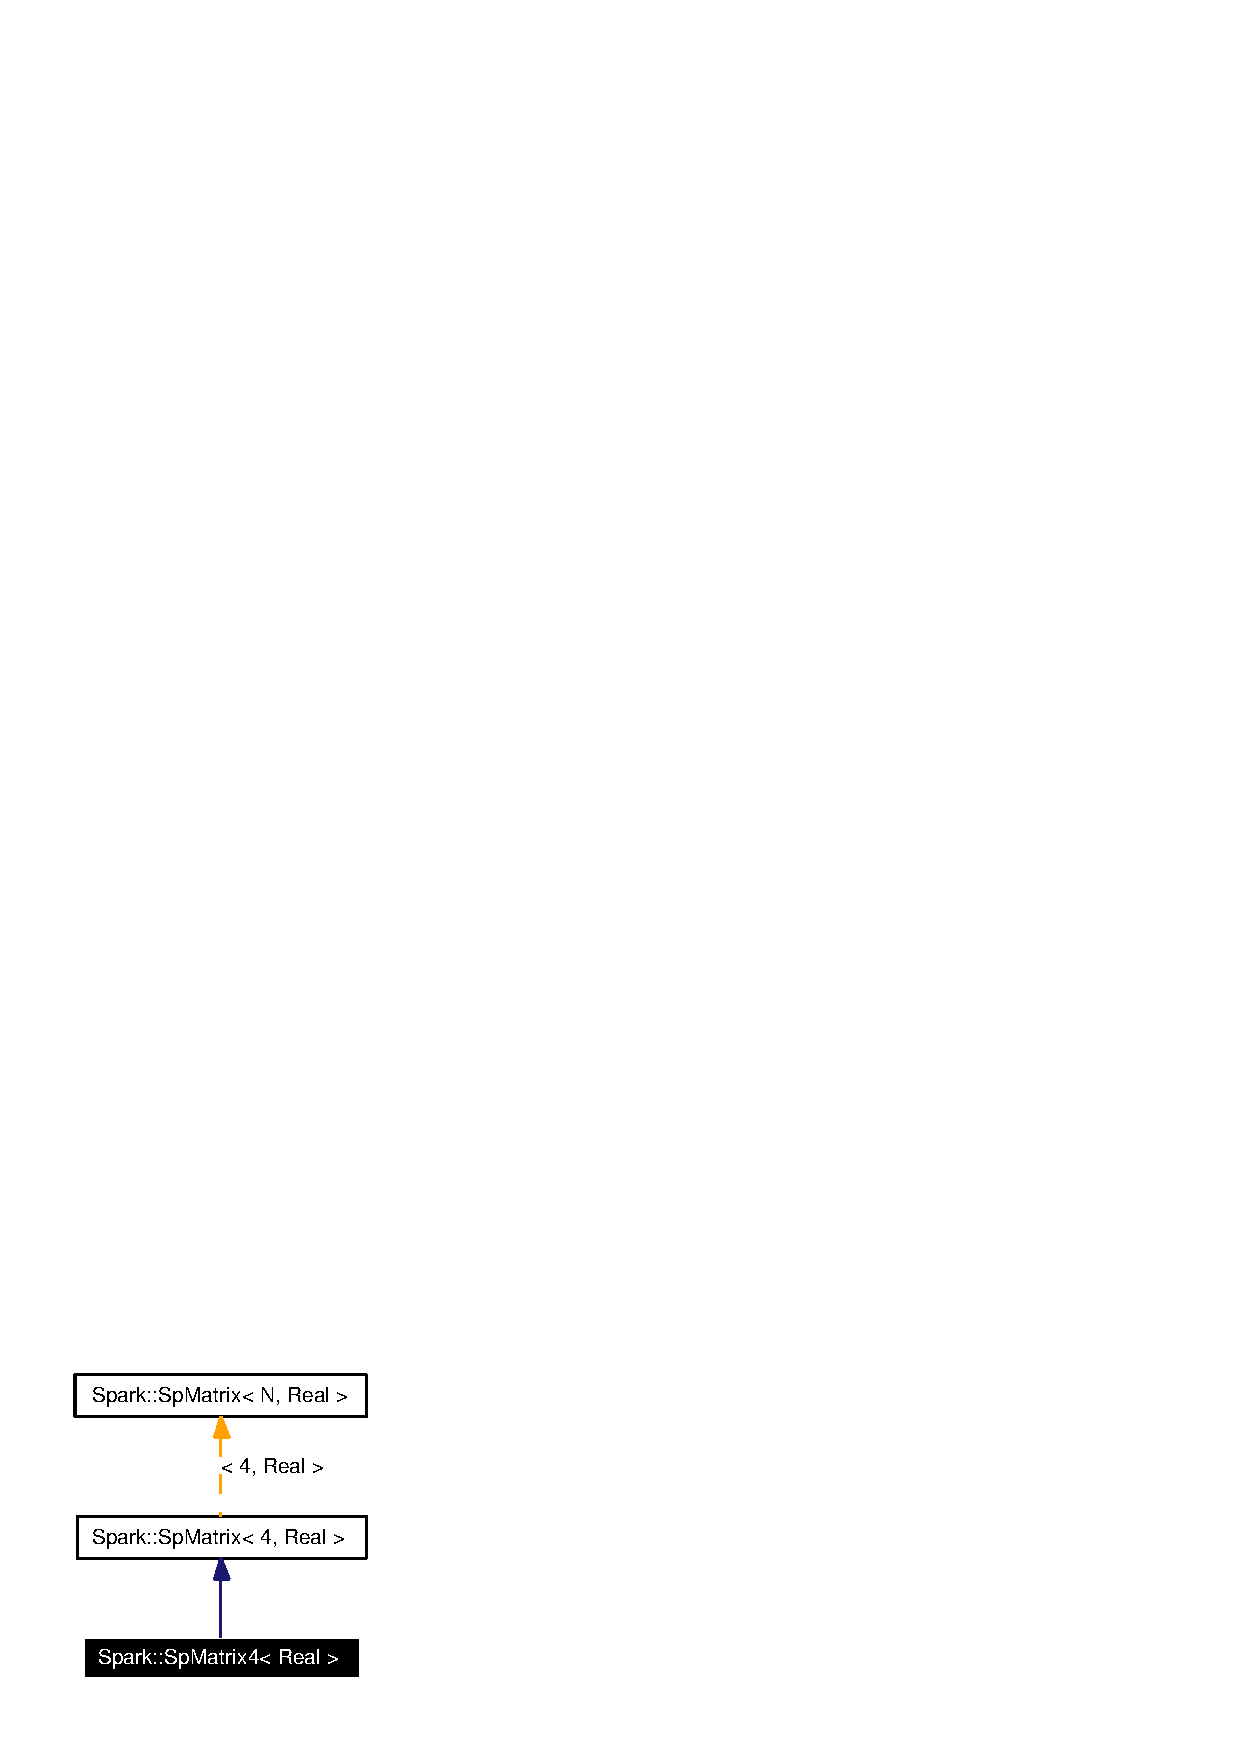
\includegraphics[width=88pt]{classSpark_1_1SpMatrix4__inherit__graph}
\end{center}
\end{figure}
Collaboration diagram for Spark::Sp\-Matrix4$<$ Real $>$:\begin{figure}[H]
\begin{center}
\leavevmode
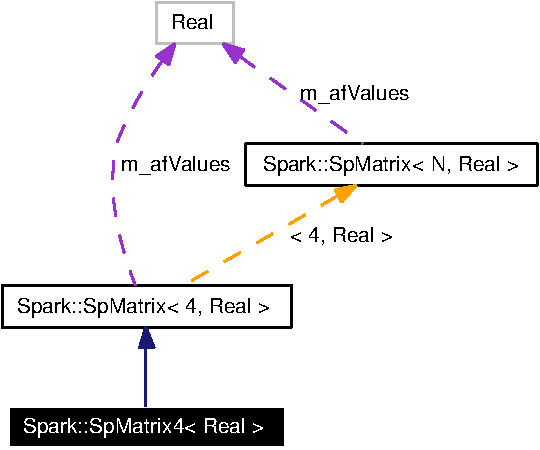
\includegraphics[width=147pt]{classSpark_1_1SpMatrix4__coll__graph}
\end{center}
\end{figure}


\subsection{Detailed Description}
\subsubsection*{template$<$class Real$>$ class Spark::Sp\-Matrix4$<$ Real $>$}

4x4 Matrix class for vector algebra 

Definition at line 169 of file Sp\-Matrix.h.\subsection*{Public Member Functions}
\begin{CompactItemize}
\item 
{\bf Sp\-Matrix4} ()
\item 
{\bf Sp\-Matrix4} (const {\bf Sp\-Matrix4} \&rk\-M)
\item 
{\bf Sp\-Matrix4} (const {\bf Sp\-Matrix}$<$ 4, Real $>$ \&rk\-M)
\item 
{\bf Sp\-Matrix4} (Real f\-M00, Real f\-M01, Real f\-M02, Real f\-M03, Real f\-M10, Real f\-M11, Real f\-M12, Real f\-M13, Real f\-M20, Real f\-M21, Real f\-M22, Real f\-M23, Real f\-M30, Real f\-M31, Real f\-M32, Real f\-M33)
\item 
{\bf Sp\-Matrix4} (const Real af\-Entry[16], bool b\-Row\-Major)
\item 
{\bf Sp\-Matrix4} \& {\bf operator=} (const {\bf Sp\-Matrix4} \&rk\-M)
\item 
{\bf Sp\-Matrix4} \& {\bf operator=} (const {\bf Sp\-Matrix}$<$ 4, Real $>$ \&rk\-M)
\end{CompactItemize}


\subsection{Constructor \& Destructor Documentation}
\index{Spark::SpMatrix4@{Spark::Sp\-Matrix4}!SpMatrix4@{SpMatrix4}}
\index{SpMatrix4@{SpMatrix4}!Spark::SpMatrix4@{Spark::Sp\-Matrix4}}
\subsubsection{\setlength{\rightskip}{0pt plus 5cm}template$<$class Real$>$ {\bf Spark::Sp\-Matrix4}$<$ Real $>$::{\bf Sp\-Matrix4} ()}\label{classSpark_1_1SpMatrix4_a0}


\index{Spark::SpMatrix4@{Spark::Sp\-Matrix4}!SpMatrix4@{SpMatrix4}}
\index{SpMatrix4@{SpMatrix4}!Spark::SpMatrix4@{Spark::Sp\-Matrix4}}
\subsubsection{\setlength{\rightskip}{0pt plus 5cm}template$<$class Real$>$ {\bf Spark::Sp\-Matrix4}$<$ Real $>$::{\bf Sp\-Matrix4} (const {\bf Sp\-Matrix4}$<$ Real $>$ \& {\em rk\-M})}\label{classSpark_1_1SpMatrix4_a1}


\index{Spark::SpMatrix4@{Spark::Sp\-Matrix4}!SpMatrix4@{SpMatrix4}}
\index{SpMatrix4@{SpMatrix4}!Spark::SpMatrix4@{Spark::Sp\-Matrix4}}
\subsubsection{\setlength{\rightskip}{0pt plus 5cm}template$<$class Real$>$ {\bf Spark::Sp\-Matrix4}$<$ Real $>$::{\bf Sp\-Matrix4} (const {\bf Sp\-Matrix}$<$ 4, Real $>$ \& {\em rk\-M})}\label{classSpark_1_1SpMatrix4_a2}


\index{Spark::SpMatrix4@{Spark::Sp\-Matrix4}!SpMatrix4@{SpMatrix4}}
\index{SpMatrix4@{SpMatrix4}!Spark::SpMatrix4@{Spark::Sp\-Matrix4}}
\subsubsection{\setlength{\rightskip}{0pt plus 5cm}template$<$class Real$>$ {\bf Spark::Sp\-Matrix4}$<$ Real $>$::{\bf Sp\-Matrix4} (Real {\em f\-M00}, Real {\em f\-M01}, Real {\em f\-M02}, Real {\em f\-M03}, Real {\em f\-M10}, Real {\em f\-M11}, Real {\em f\-M12}, Real {\em f\-M13}, Real {\em f\-M20}, Real {\em f\-M21}, Real {\em f\-M22}, Real {\em f\-M23}, Real {\em f\-M30}, Real {\em f\-M31}, Real {\em f\-M32}, Real {\em f\-M33})}\label{classSpark_1_1SpMatrix4_a3}


\index{Spark::SpMatrix4@{Spark::Sp\-Matrix4}!SpMatrix4@{SpMatrix4}}
\index{SpMatrix4@{SpMatrix4}!Spark::SpMatrix4@{Spark::Sp\-Matrix4}}
\subsubsection{\setlength{\rightskip}{0pt plus 5cm}template$<$class Real$>$ {\bf Spark::Sp\-Matrix4}$<$ Real $>$::{\bf Sp\-Matrix4} (const Real {\em af\-Entry}[16], bool {\em b\-Row\-Major})}\label{classSpark_1_1SpMatrix4_a4}




\subsection{Member Function Documentation}
\index{Spark::SpMatrix4@{Spark::Sp\-Matrix4}!operator=@{operator=}}
\index{operator=@{operator=}!Spark::SpMatrix4@{Spark::Sp\-Matrix4}}
\subsubsection{\setlength{\rightskip}{0pt plus 5cm}template$<$class Real$>$ {\bf Sp\-Matrix4}\& {\bf Spark::Sp\-Matrix4}$<$ Real $>$::operator= (const {\bf Sp\-Matrix}$<$ 4, Real $>$ \& {\em rk\-M})}\label{classSpark_1_1SpMatrix4_a6}


\index{Spark::SpMatrix4@{Spark::Sp\-Matrix4}!operator=@{operator=}}
\index{operator=@{operator=}!Spark::SpMatrix4@{Spark::Sp\-Matrix4}}
\subsubsection{\setlength{\rightskip}{0pt plus 5cm}template$<$class Real$>$ {\bf Sp\-Matrix4}\& {\bf Spark::Sp\-Matrix4}$<$ Real $>$::operator= (const {\bf Sp\-Matrix4}$<$ Real $>$ \& {\em rk\-M})}\label{classSpark_1_1SpMatrix4_a5}




The documentation for this class was generated from the following file:\begin{CompactItemize}
\item 
{\bf Sp\-Matrix.h}\end{CompactItemize}
